\section{Related Work}\label{relatedWork}
%Camera Path Animator 3.0 (Unity asset store).
%Camera system that follows the character but also focuses on showing the environment - Used in the game God of War.

\begin{figure*}[htbp]
\centering
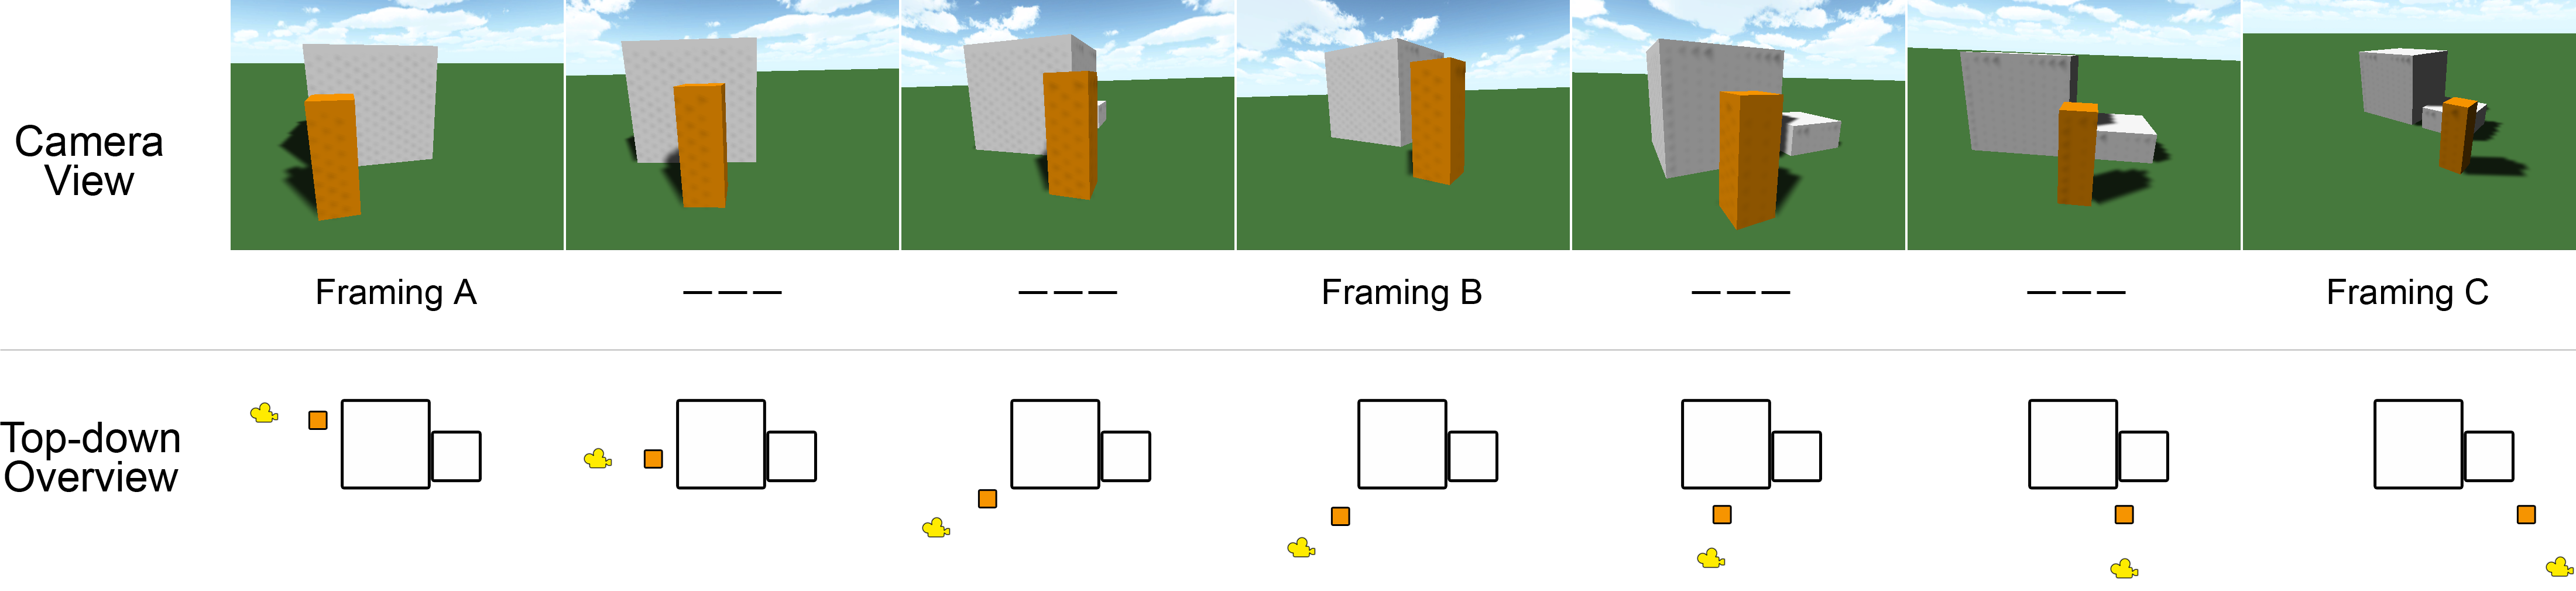
\includegraphics[width=1\textwidth]{Pics/InterpolationExample}
\caption{An example of a camera interpolation between three framings (A, B and C). The framings contain position, rotation and field of view. As the player character (orange cube) moves, the camera follows him by interpolating between the framings.}
\label{fig:InterpolationExample}
\end{figure*}

The main requirements of a camera tool in most games is that it can go from position one position (A) to another  position (B) depending on player position or certain events. For instance, A and B can be different in position, rotation and field of view.
%By looking at games with emphasis on its visuals and environments, it was found that the camera changes its position, rotation and field of view. 
Figure \ref{fig:InterpolationExample} shows an example of how the camera interpolates between three positions.

%\begin{figure}[htbp]
%\centering
%
\includegraphics[width=.4\textwidth]{Pics/CameraSystem_BASIC}
%\caption{The camera interpolates between position A and B. A and B contain information about its %position, rotation and field of view.}
%\label{fig:CameraSystem_BASIC}
%\end{figure}

\subsection{Camera Tools}

During initial research, we found a tool called Camera Path Animator 3.0 by Jasper Stocker  \cite{unity_camTool}. It can be used for creating animated cameras within Unity. As the name suggests, it works by animating the camera along a specified path, which can have various shapes (e.g., Bezier and Hermite curves). The tool is primarily targeted towards creating cameras that move linearly along a set path, i.e. for use in cinematic sequences. It provides various ways of inserting, moving and deleting points, as well as changing settings such as field of view, speed, interpolation type and easing. Additionally, it has a event system for triggering certain events at certain points in the path.

%\begin{figure}[htbp]
%\centering
%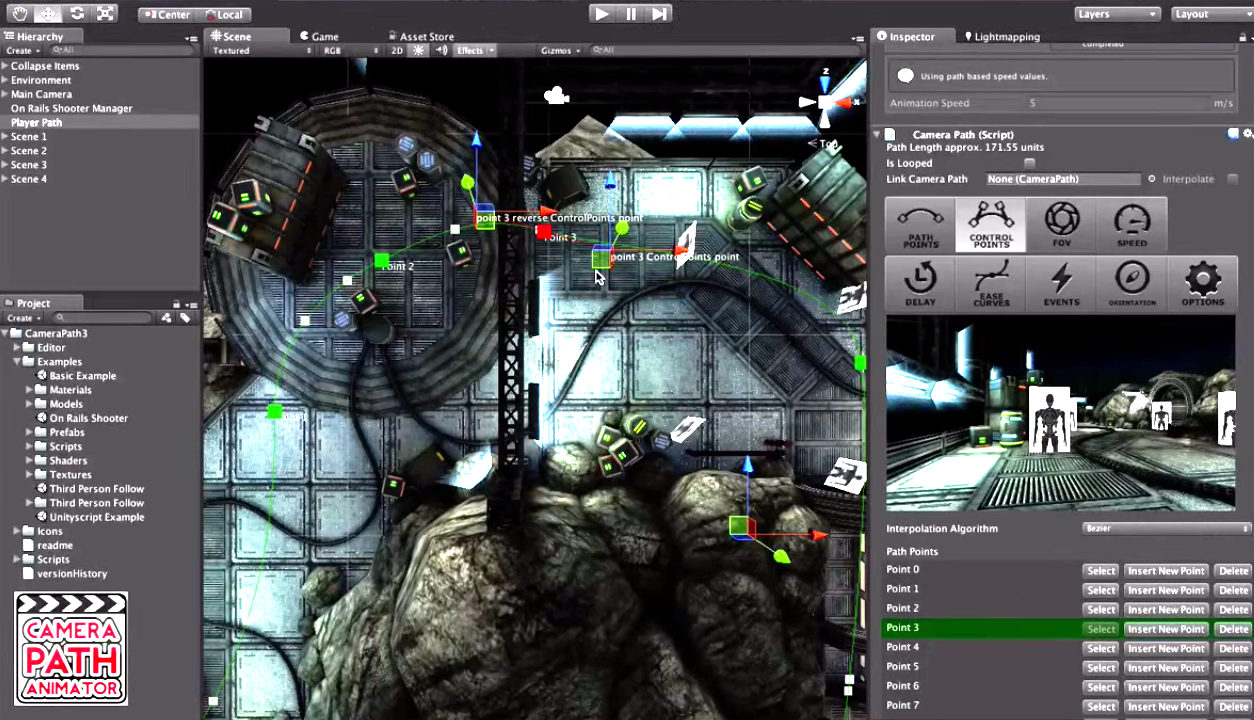
\includegraphics[width=0.40\textwidth]{Pics/unity_path_cam_tool}
%\caption{Overview of the objects related to the camera system.}
%\label{fig:unity_path_cam_tool}
%\end{figure}

%The God of War video game franchise for the PlayStation systems has also made notable use of their camera systems. The developers call the system Rail Driven Cameras and consists of a 'rail' that will be placed in the game world. A camera is keyed in both ends of the rail, and the camera will then animate between them as the protagonist moves along the rail. % Det her føles pølse, ikke meget at skrive om det og super unscientific

\begin{figure}[htbp]
\centering
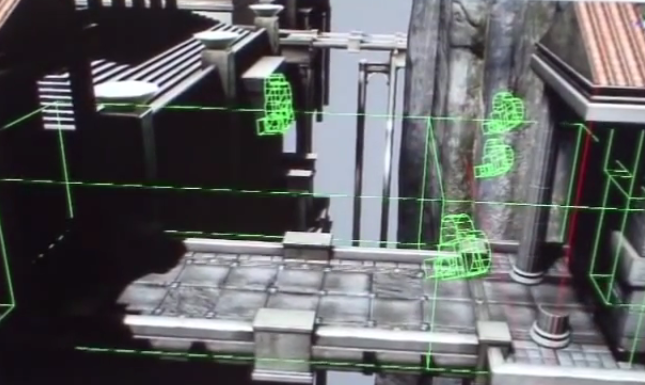
\includegraphics[width=0.45\textwidth]{Pics/gow_cameraZones}
\caption{Depending on what zone the player is located in, certain cameras are activated. \protect\cite{gow_camera}}
\label{fig:gow_zones}
\end{figure}

In a behind-the-scenes documentary, the developers behind the PlayStation game series \textit{God of War}, Santa Monica Studio, talks about the importance of being able to frame the scene \cite{gow_camera}. Depending on the context, it is important for them to frame the scene, so players know where they should be heading next. They use camera zones to determine what area the player is in and then activate the corresponding camera for that zone (see Figure \ref{fig:gow_zones}).

%\begin{figure}[htbp]
%\centering
%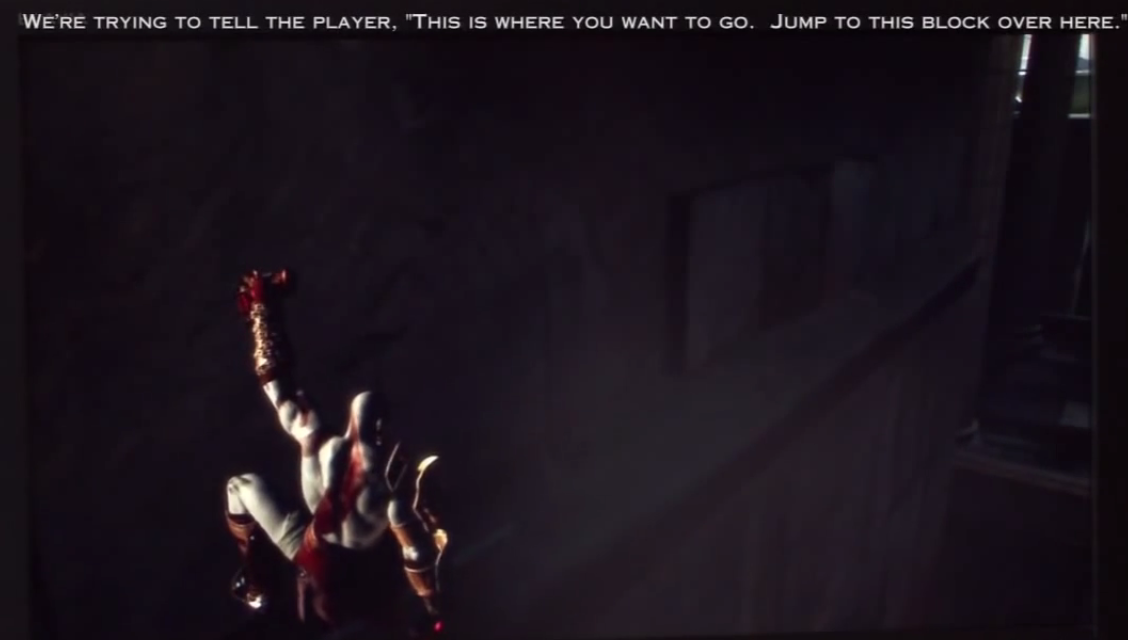
\includegraphics[width=0.40\textwidth]{Pics/gow_next}
%\caption{The camera's framing can help the designer guide the player in the right direction.}
%\label{fig:gow_jump}
%\end{figure}


%An example of this is when the main character has to jump from one 

\subsection{Participatory Design}
Participatory design (PD) has been defined as the participation of users in the design process of a system that is to be implemented in an organization (INSERT REF). Here, users correspond to workers in the organization. By involving users in the design, their skills, experiences, and interests are taken into consideration, thereby increasing the likelihood that the system will be useful to them.

According to PD researchers, it is important there is an active cooperation between the designer and the user(INSERT REF). This results in the designer gaining knowledge of the user's current work practices, and the user gaining knowledge of the technology to be used. It is also important that users take an active part in the analysis of needs, selection of technology, design and prototyping, as well as organizational implementation.